
\documentclass[
12pt, % Main document font size
a4paper, % Paper type, use 'letterpaper' for US Letter paper
oneside, % One page layout (no page indentation)
%twoside, % Two page layout (page indentation for binding and different headers)
headinclude,footinclude, % Extra spacing for the header and footer
BCOR5mm, % Binding correction
]{scrartcl}

%%%%%%%%%%%%%%%%%%%%%%%%%%%%%%%%%%%%%%%%%
% Arsclassica Article
% Structure Specification File
%
% This file has been downloaded from:
% http://www.LaTeXTemplates.com
%
% Original author:
% Lorenzo Pantieri (http://www.lorenzopantieri.net) with extensive modifications by:
% Vel (vel@latextemplates.com)
%
% License:
% CC BY-NC-SA 3.0 (http://creativecommons.org/licenses/by-nc-sa/3.0/)
%
%%%%%%%%%%%%%%%%%%%%%%%%%%%%%%%%%%%%%%%%%

%----------------------------------------------------------------------------------------
%	REQUIRED PACKAGES
%----------------------------------------------------------------------------------------

\usepackage[
nochapters, % Turn off chapters since this is an article        
beramono, % Use the Bera Mono font for monospaced text (\texttt)
eulermath,% Use the Euler font for mathematics
pdfspacing, % Makes use of pdftex’ letter spacing capabilities via the microtype package
dottedtoc % Dotted lines leading to the page numbers in the table of contents
]{classicthesis} % The layout is based on the Classic Thesis style

\usepackage{arsclassica} % Modifies the Classic Thesis package

\usepackage[T1]{fontenc} % Use 8-bit encoding that has 256 glyphs

\usepackage[utf8]{inputenc} % Required for including letters with accents

\usepackage{graphicx} % Required for including images
\graphicspath{{Figures/}} % Set the default folder for images

\usepackage{enumitem} % Required for manipulating the whitespace between and within lists

\usepackage{lipsum} % Used for inserting dummy 'Lorem ipsum' text into the template

\usepackage{subfig} % Required for creating figures with multiple parts (subfigures)

\usepackage{amsmath,amssymb,amsthm} % For including math equations, theorems, symbols, etc

\usepackage{varioref} % More descriptive referencing

%----------------------------------------------------------------------------------------
%	THEOREM STYLES
%---------------------------------------------------------------------------------------

\theoremstyle{definition} % Define theorem styles here based on the definition style (used for definitions and examples)
\newtheorem{definition}{Definition}

\theoremstyle{plain} % Define theorem styles here based on the plain style (used for theorems, lemmas, propositions)
\newtheorem{theorem}{Theorem}

\theoremstyle{remark} % Define theorem styles here based on the remark style (used for remarks and notes)

%----------------------------------------------------------------------------------------
%	HYPERLINKS
%---------------------------------------------------------------------------------------

\hypersetup{
%draft, % Uncomment to remove all links (useful for printing in black and white)
colorlinks=true, breaklinks=true, bookmarks=true,bookmarksnumbered,
urlcolor=webbrown, linkcolor=RoyalBlue, citecolor=webgreen, % Link colors
pdftitle={}, % PDF title
pdfauthor={\textcopyright}, % PDF Author
pdfsubject={}, % PDF Subject
pdfkeywords={}, % PDF Keywords
pdfcreator={pdfLaTeX}, % PDF Creator
pdfproducer={LaTeX with hyperref and ClassicThesis} % PDF producer
} % Include the structure.tex file which specified the document structure and layout

\hyphenation{Fortran hy-phen-ation} % Specify custom hyphenation points in words with dashes where you would like hyphenation to occur, or alternatively, don't put any dashes in a word to stop hyphenation altogether

%----------------------------------------------------------------------------------------
%	TITLE AND AUTHOR(S)
%----------------------------------------------------------------------------------------

\title{\normalfont\spacedallcaps{Research Proposal}} % The article title

%\subtitle{Subtitle} % Uncomment to display a subtitle

\author{\spacedlowsmallcaps{Jin Choi\textsuperscript{*}}} % The article author(s) - author affiliations need to be specified in the AUTHOR AFFILIATIONS block

\date{} % An optional date to appear under the author(s)

%----------------------------------------------------------------------------------------

\begin{document}

%----------------------------------------------------------------------------------------
%	HEADERS
%----------------------------------------------------------------------------------------

\renewcommand{\sectionmark}[1]{\markright{\spacedlowsmallcaps{#1}}} % The header for all pages (oneside) or for even pages (twoside)
%\renewcommand{\subsectionmark}[1]{\markright{\thesubsection~#1}} % Uncomment when using the twoside option - this modifies the header on odd pages
\lehead{\mbox{\llap{\small\thepage\kern1em\color{halfgray} \vline}\color{halfgray}\hspace{0.5em}\rightmark\hfil}} % The header style

\pagestyle{scrheadings} % Enable the headers specified in this block

%----------------------------------------------------------------------------------------
%	TABLE OF CONTENTS & LISTS OF FIGURES AND TABLES
%----------------------------------------------------------------------------------------

\maketitle % Print the title/author/date block

\setcounter{tocdepth}{2} % Set the depth of the table of contents to show sections and subsections only

\tableofcontents % Print the table of contents

\listoffigures % Print the list of figures

\listoftables % Print the list of tables

%----------------------------------------------------------------------------------------
%	AUTHOR AFFILIATIONS
%----------------------------------------------------------------------------------------

\let\thefootnote\relax\footnotetext{* \textit{Department of Physics and Astronomy, Seoul National University, Seoul, Republic of Korea}}

%----------------------------------------------------------------------------------------

\newpage % Start the article content on the second page, remove this if you have a longer abstract that goes onto the second page

%----------------------------------------------------------------------------------------
%	INTRODUCTION
%----------------------------------------------------------------------------------------

\section{Introduction}

In 2012, a spin 0 particle with its mass of 125 GeV has been discovered\cite{ATLASHiggsDiscovery}\cite{CMSHiggsDiscovery},
which can be interpreted as Higgs Boson($H$) in the Standard Model(SM)\cite{StandardModel}.
The discovery of the particle completed the theory, but there are still many anomalies
that cannot be explained in SM. For example, the mass hierachy problem, matter-antimatter
asymmetry, or the existence of the dark matter are still not understood well yet. Therefore, many
theories so called Beyond the Standard Model(BSM) have been constructed and many of them
extend the singlet Higgs sector to be doublet. In general two Higgs doublet model(2HDM)\cite{2HDM}, the
theory predicts 5 physical Higgs eigenstates: two charged Higgs bosons($H^{\pm}$),
two neutral Higgs bosons($H$, $h$), and one pseudoscalar Higgs boson($A$).
The already founded particle can be one of the neutral Higgs boson, so if it is the light neutral
Higgs boson, then it is called normal scenario(NS), otherwise inverted scenario(IS).

Since there are no mass relation in 5 physical eigenstats of the Higgs bosons, various decay modes
of $H^{\pm}$ can be established. The most actively searched decay modes 
in the LHC are fermionic decay modes such as
$H^+ \rightarrow t\bar{b}$\cite{HcTotb}, 
$H^+ \rightarrow c\bar{s}$\cite{HcTocs}, and 
$H^+ \rightarrow \tau^+\nu$\cite{HcTotaunu}.
These channels are used to set upper limits on the mass of $H^+$ and $tan\beta$, 
depending on the type of each 2HDM model.
There are also bosonic decay modes\cite{BosonicDecay} such as
$H^+ \rightarrow hW^+$,
$H^+ \rightarrow HW^+$, and
$H^+ \rightarrow W^+A$.
Especially, $H^{\pm}W^{\mp}A$ coupling does not depend on $tan\beta$,
so if it is kinematically allowed, $H^+ \rightarrow W^+A$ can be the most dominant
decay mode and highly suppress the fermionic decay modes\cite{HcToWASearch}.
The importance of the $H^+ \rightarrow W^+A$ decay mode was well known in the LEP era.
The DELPHI and OPAL experiment set the lower bound in the $m_{H^+}$ at 72 GeV
in type 1 2HDM with $m_A \in$[12, 70] GeV using $e^+e^- \rightarrow H^+H^-$ production\cite{DELPHISearch}\cite{OPALSearch}.
In Tevatron, the CDF experiment searched the
$H^+ \rightarrow W^+a \rightarrow W^+\tau^+\tau^-$
decay mode with $m_{H^+} \in$ [90, 160] GeV and $m_A \in$ [4, 9] GeV,
setting the upper limit on the branching fraction 
$B(t \rightarrow bH^+ \rightarrow bW^+a \rightarrow bW^+\tau^+\tau^-)$
as 8 to 50\%\cite{CDFSearch}. At the LHC Run1, there was no search for $H^+ \rightarrow W^+A$ decay mode,
but the Atlas experiment searched another bosonic decay mode $H^+ \rightarrow W^+Z$. In Run 2,
only the CMS  experiment searched $H^+ \rightarrow W^+A$ decay mode from top quark pair production 
using $35.9 fb^{-1}$ data collected in 2016. The research have set the upper limit on
$B(t \rightarrow bH^+ \rightarrow bW^+A \rightarrow bW^+\mu^+\mu^-) \le$ 2.9\% at 95\% CL,
assuming $m_{H^+} \in$ [70, 160] GeV and $15 GeV < m_A < m_t - m_{H^+}$\cite{PreviousSearch}.

In this research, we will use the full Run2 LHC data collected by the CMS experiment
to enhance the sensitivity searched in the previous analysis.
In addition, we will investigate the off-shell decay of $H^+ \rightarrow W^+A$ decay mode 
($m_{H^+} < m_A + m_{W^+})$. Previous searches have been avoided this 
pseudoscalar Higgs mass region because of the large background from Z associated productions(e.g. $t\bar{t}+Z$),
but increased number of events and using novel MVA methods made the search possible.

\section{Data and Simulated samples}
LHC full Run2 proton-proton collision data, which is total integrated luminosity of 139$fb^-1$, 
collected by the CMS experiments is used in this analysis.
The data has been triggered by either doublemuon triggers or electron-muon triggers depending on
the final state leptons as described in section 4. More detail description of the CMS detector and
the triggering system can be found in Ref. \cite{Detector} \cite{Trigger}.

The signal events are generated using Madgraph\_aMC@NLO v5.2.6.5\cite{Madgraph} in leading order. 
General 2HDM model cards restricted by type 1 scenario has been used. 
The mass of the heavy Higgs boson is set to be 5TeV to avoid its production or decay, 
while the mass of the light Higgs boson is set to be $125$ GeV.
The mass of charged Higgs boson is set to be between $70$ GeV and $160$ GeV, 
and the mass of the pseudoscalr Higgs boson is set to be between $15$ GeV and $m_{H^+} - 5$ GeV. 
Each sample is normalized to $15fb$.
Background samples are generated using Powheg Box v2\cite{Powheg} or Madgraph\_aMC@NLO v5.2.6.5\cite{Madgraph} 
up to leading order(LO) or next-leading order(NLO) in matrix element calculation, 
and some samples are normalized up to higher order precision.
More information of the background sample generation can be found in Table 1.
For all samples, the actual detection process was implemented through Geant4 detector simulation\cite{Geant4}.


\begin{table}[hbt]
    \caption{Background Samples}
    \centering
    \begin{tabular}{llll}
        \toprule
        Sample  & ME Generator    & Xsec($pb$)    & Precision \\
        \midrule
        TTLL & Powheg & $88.29$ & NNLO \\
        Z+jets & MC@NLO & $6077.22$ & NNLO \\
        WZ $\rightarrow$ 3$l\nu$ & MC@NLO & $5.213$ & NLO \\
        ZZ $\rightarrow$ 4$l$ & Powheg & $1.256$ & NLO \\
        Z$\gamma \rightarrow ll\gamma$ & MC@NLO & $51.1$ & NLO \\
        TT+W (W $\rightarrow l\nu$) & MC@NLO & $0.2043$ & NLO \\
        TT+Z (Z $\rightarrow 2l2\nu$) & MC@NLO & $0.2529$ & NLO \\
        TT+H (H $\nrightarrow$ bb) & Powheg & $0.2151$ & NNLO QCD+NLO EW \\
        tZq & MC@NLO & $0.0758$ & NLO \\
        tHq & Madgraph & $0.7464$ & LO \\
        VVV(V = W, Z) & MC@NLO & $0.44333$ & NLO \\
        TTTT & MC@NLO & $0.009103$ & NLO \\
        VBF H$\rightarrow$ZZ$\rightarrow$4$l$ & Powheg & $0.001034$ & NLO \\
        ggH$\rightarrow$ZZ$\rightarrow$4$l$ & Powheg & $0.01212$ & NLO \\
        \bottomrule
    \end{tabular}
    \label{tab:label}
\end{table}

\section{Object Definition}
Final objects are reconstructed by particle flow(PF) algorithm\cite{ParticleFlow}, which not only use the subdetector
information but use all the subdetector information for better identify the final objects.
The major objects we use in this analysis is electrons, muons, and jets. Electrons use tracker to measure
it's position and momentum combined with the ECAL information\cite{Electron}. Tracks that matched to the muon stations
can be identified as muons\cite{Muon}. Other objects, such as charged hadrons, neutral hadrons or tau lepton can also be identified,
while neutrinos escape from the detector but it's transverse momentum can be measured as negative vector sum of the $p_{T}$ of all the
PF candidates. Jets use all the PF candidates using anti-kt algorithm\cite{AntiKT} with cone size of 0.4.
To identify b-jets, all the constituents are used to train the tagger\cite{DeepJet}, which gives scores to be light, c or b.
Here, b-tagged jets are called b-jets.

\section{Search Strategy}
In this analysis, we investigate $H^+$ and $A$ with the mass range of
70 GeV < $m_{H^+}$ < 160 GeV and 15 GeV < $m_A$ < $m_H^+$ - 5 GeV using 139 $fb^{-1}$
of proton-proton collision data at $\sqrt{s}$ = 13 TeV collected during the LHC Run 2
by the CMS experiment. Here, the mass of $H^+$ has been set to be greater than the lower bound
from LEP experiment and less than that of the top quark. The mass of $A$ has been set to avoid
the low mass resonances but allow the off-shell decay from $H^+$. The most dominant
charged Higgs production channel in this mass range is through top quark pair production, and we search for the 
cascade decay chain $H^+ \rightarrow W^+A \rightarrow W^+\mu^+\mu^-$. Assuming at least one
of the $W$ bosons decay leptonically, the final state contains $e\mu\mu$ of $\mu\mu\mu$ + multijet + b-tagged jet
signature. The Feynman diagram of the signal event has been shown in figure 1. 
The dominant background in this channel is leptonically decaying top quark pair production, 
with one of the jets being misidentified as a muon or an electron(non-prompt background).
Prompt contribution from $WZ \rightarrow 3l + \nu$ and $ZZ \rightarrow 4l$(VV), $TT + X(X=W, Z, H)$
are also contributed to the dominant background sources. Drell-Yan processes with bremsstrahlung
of final state leptons, referred to as conversion background, are also estimated. Some rare processes
such as $H \rightarrow ZZ \rightarrow 4l$ with $H$ produced either by gluon fusion or vector boson fusion,
$VVV (V=W, Z)$, $TTTT$ are also considered.

\begin{figure}[htp]
    \centering
    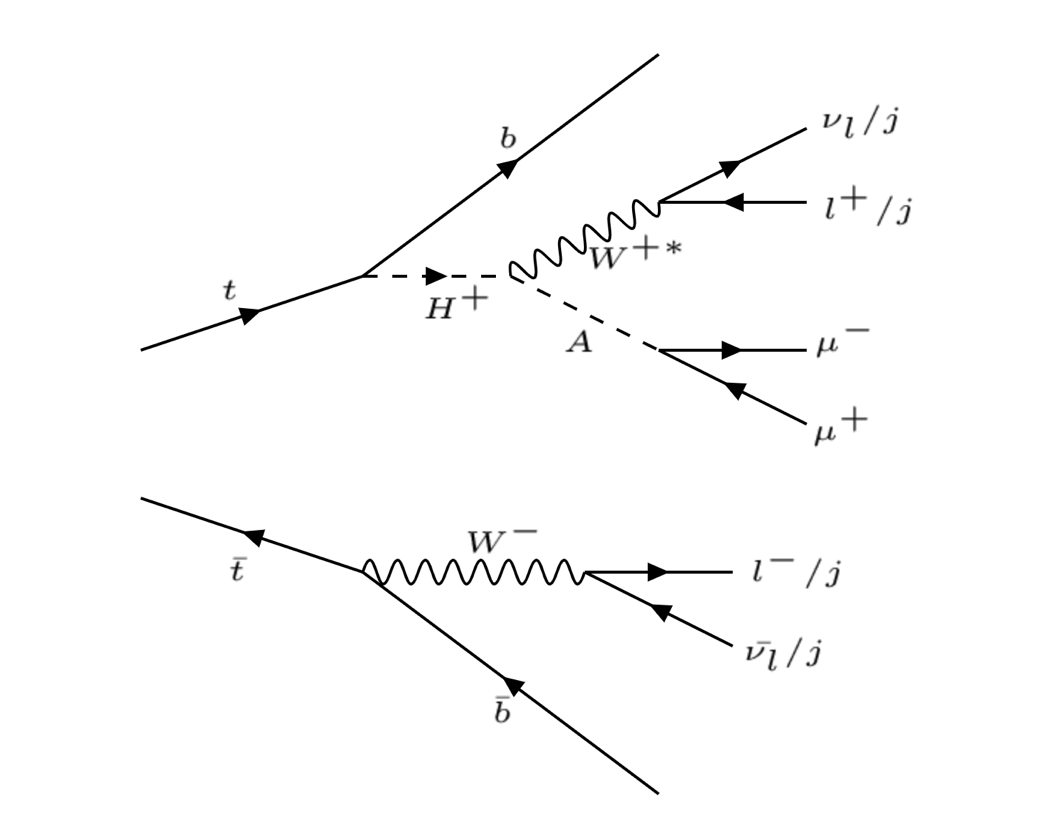
\includegraphics[width=8cm]{FeynmanDiagram.png}
    \caption{Feynman diagram for the signal events.}
    \label{fig:Feynman}
\end{figure}

Baseline selection of events has been build based on the signal event topology.
If $m_{H^+}$ ~ $m_t$, b-jets branching from the top quark associated with the charged Higgs
can be very soft. Not to loose such signal events, instead of requiring 2 b-jets, we only require
single b-jet. The final baseline selection is as below:
\begin{itemize}
    \item 3 muons \ 1 electron + 2 muons with at least one OS muon pair
    \item least two jets
    \item at least one b-tagged jet
\end{itemize}

By using the opposite signed muon pair, it is easy to reconstruct the pseudoscalar candidates.
However, to reconstruct the charged Higgs candidate is not a simple job. Instead of reconstructing
the charged Higgs, we decided to use the final objects' kinematics 
to discriminated irreducible background further.
Graph-neural-network(GNN) based discriminators\cite{GNN}\cite{ParticleNet} are trained to separate the signal events 
and the nonprompt or $TT + X$ backgrounds. 
To make the network sensitive to the final states' kinematics, Graph based data structure
is the most natural way to represent the data, since the graph is length-free and permutation invariant data structure.
Here, we only used $P_T$, $\eta$, $\phi$, mass, charge, PID(=muons, electrons, jets), b-tag score for the discrimination.
Other ML techniques such as boosted decision tree(BDT) or deep neural network(DNN) frequently use high-level
features constructed from several objects and represent an event
as a list, which have to assume a manual ordering(e.g. PT ordering in jets) and have to drop some information or
zero-padded the list to avoid the blank in the list.
In GNN, each object in an event can be represented as a node and their relation such as $\Delta R$ or reconstructed mass
can be represented in the edge attribute of two objects. The network convolute the nearby objects and generate a new graph
with different number of node attributes and edge attributes. The information of the final graph is aggregated in the readout
layers and make a fixed length of list, so can be flow to the final probability, which is the score to be a signal event.

The event rate for each background source is measured in a different manner.
For the nonprompt background, the contribution is estimated using tight-loose method from the data. 
In this method, we use single lepton events to measure the probability of nonprompt leptons passing the loose ID but not tight ID. 
The probability is used to estimate the expected event rate in the application regions 
by extrapolating the event rates that not all the leptons passing the tight ID. 
For the conversion background, since the MC modelling of the conversion leptons might be ill-modelled, 
the scale factors for $Z+\gamma$ samples are measured in the separated control region 
which is dominated by $Z+\gamma$ events and orthogonal to the baseline selection.
The other prompt backgrounds such as $VV$ or $TT + X$ are estimated directly from the MC samples.

In the final sensitivity calculation, the most dominant backgrounds, 
TT+nonprompt and $VV$, $TT + X$, 
will be suppressed using the GNN response of each event.
The final limit will be extracted using the dimuon mass spectrum, which is the candidate
of the pseudoscalar Higgs boson.
The result will be interpreted as the signal production rate in each mass point using profile likelihood method\cite{limit}.

\section{Current Status and Future Plans}
In this analysis, electrons, muons, and jets are used to describe the events.
The object definition are finalized. For muons, measuring the ID efficiency in
data and simulation has been done with corresponding trigger efficiency, and
the correction factor has been applied to each MC samples to describe the data better.
Also, the nonprompt probability has been measure to estimate the nonprompt background
using tight-loose method. For electrons, even if the definition for tight and loose ID
criteria has been finalized, its efficiency and nonprompt probability have not been measured yet.
Jets and missing transverse momenta definitions are provided from the CMS central POG team.

Since we have not measured the correction factors and nonprompt probability of electrons yet,
training the GNN discriminator for $\mu\mu\mu$ channel has been done in first. We will use the
discrimination score and the dimuon mass spectrum to check the preliminary sensitivity soon.

After measuring the electron efficiency and nonprompt probability, the result from $e\mu\mu$
channel will be supplemented. Also, systematic sources have not been considered properly,
for example the b-tagging efficiency correction for jet energy resolution. It will also be
accounted in the final interpretation.

The result will be published in the name of CMS collaboration within an year.

%----------------------------------------------------------------------------------------
%	BIBLIOGRAPHY
%----------------------------------------------------------------------------------------

\renewcommand{\refname}{\spacedlowsmallcaps{References}} % For modifying the bibliography heading

\bibliographystyle{unsrt}

\bibliography{sample.bib} % The file containing the bibliography

%----------------------------------------------------------------------------------------

\end{document}